\section{Theorie}
\label{sec:Theorie}


\subsection{Die Strahlungsleistung des elektromagnetischen Feldes}

Für die Herleitung die Winkelabhängkeit der Intensität werden zunächst die Maxwellgleichngen
\begin{align*}
    \nabla \times \vec{H}=\vec{j}+\varepsilon \varepsilon_{0} \frac{ \dif{\vec{E}}}{ \dif{t}} 
    \quad & \text{und} \quad 
    \nabla \times \vec{E}=-\mu \mu_{0} \frac{\dif{\vec{H}}}{\dif{t}} 
\end{align*}
betrachtet. Die elektrische und magnetische Arbeit
\begin{align*}
    W_{\text{el}}   :=  \frac{1}{2} \varepsilon \varepsilon_{0} \vec{E}^{2} 
    \quad & \text{und} \quad 
    W_{\text{mag}}  :=  \frac{1}{2} \mu_{0} \vec{H}^{2}
\end{align*}
stellen dabei die Energie der Strahlungsleistung pro Volumeneinheit dar.
Der Energietransport wird dabei durch den \textit{Poynting-Vektor} 
\begin{align} \label{eq:poynting}
    \vec{S}= \vec{E} \times \vec{H}
    \quad & \text{und} \quad
    |\vec{S}|= v \varepsilon \varepsilon_{0} \vec{E}^{2}
\end{align}
beschrieben.


\subsection{Berechnung der Amplitude einer reflektierten Lichtwelle}

Fällt nun eine ebene Lichtwelle der Form
\begin{align}
    \vec{E} = \vec{E}_\text{e} \cdot e^{i \left( \vec{k} \vec{r} - \omega t \right)}
\end{align}
aus dem Vakuum unter dem Winkel $\alpha$ auf eine Grenzfläche,
wird ein Teil der Strahlung mit der Amplitude $\vec{E}_\text{r}$ reflektiert,
während der der andere mit der Amplitude $\vec{E}_\text{d}$ in das Medium eindringt.
Dieser Prozess ist in \autoref{fig:grenzflaeche1} dargestellt wird als absorptionsfrei angenommen.
\begin{figure}
    \centering
    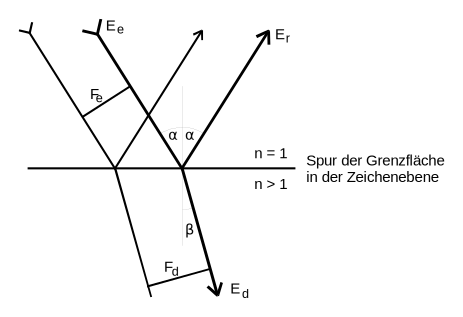
\includegraphics[width=0.8\linewidth]{pictures/grenzfläche1.pdf}
    \caption{Reflexion und Brechung der ebenen Lichtwelle. \cite{v407}}
    \label{fig:grenzflaeche1}
\end{figure}

Da die Lichtgeschwindigkeit im Medium geringer ist als im Vakuum,
ändert der eindringende Lichtstrahl seine Richtung, sodass $\beta < \alpha$ gilt.
Dadurch ergibt sich auch eine Querschnittänderung des Strahlenbündels von $F_\text{e}$ und $F_\text{d}$.
Dem Energiesatz nach gilt
\begin{align} \label{eq:energiesatz1}
    S_\text{e} F_\text{e} &= S_\text{r} F_\text{e} + S_\text{d} F_\text{d} \\
    \intertext{oder}
    S_\text{e} \cos(\alpha) &= S_\text{r} \cos(\alpha) + S_\text{d} \cos(\beta) \, .
\end{align}
Nach Einsetzen der \autoref{eq:poynting} für die Strahlungsleistung ergibt sich für \autoref{eq:energiesatz1} 
\begin{equation} \label{eq:energiesatz2}
    \text{c} \varepsilon_{0} \vec{E}_{\text{e}}^{2} \cos(\alpha) = \text{c} \varepsilon_{0} \vec{E}_{\text{r}}^{2} \cos(\alpha) + v \varepsilon \varepsilon_{0} \vec{E}_{\text{d}}^{2} \cos(\beta) \, .
\end{equation}
Mithilfe des Brechungsindex und der Maxwellschen Relation
\begin{align*}
    n = \frac{\text{c}}{v} \quad \text{und} \quad n^2 = \varepsilon
\end{align*}
kann \autoref{eq:energiesatz2} als
\begin{equation} \label{eq:energiesatz3}
    \left( \vec{E}_{\text{e}}^{2} - \vec{E}_{\text{r}}^{2} \right) \cos(\alpha) = n \vec{E}_{\text{d}}^{2} \cos(\beta)
\end{equation}  
ausgedrückt werden. 
Dabei setzt sich die eingehende Welle $\vec{E}_\text{e}$ aus einem parallelen und senkrechten Teil zusammen.
\begin{equation}
    \vec{E}_{e}=\vec{E}_{\|}+\vec{E}_{\perp}
\end{equation}
Aufgrund des unterschiedlichen Verhaltens wer Wellen an der Grenzfläche, werden diese zunächst getrennt betrachtet.


\subsection{Reflexion des senkrechten polarisierten Lichtstrahls}

In \autoref{fig:grenzflaeche2} ist die Reflexion des senkrecht polarisierten Lichts dargestellt.
\begin{figure}[ht]
    \centering
    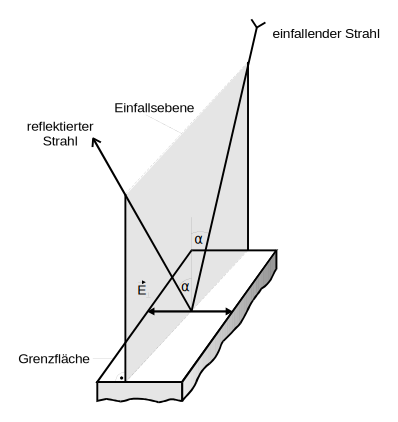
\includegraphics[width=0.7\linewidth]{pictures/grenzfläche2.pdf}
    \caption{Reflexion und Brechung des senkrecht polarisierten Lichtstrahls. \cite{v407}}
    \label{fig:grenzflaeche2}
\end{figure}

Da die Tangentialkomponente des Feldstärkevektors stetig durch die Grenzfläche geht,
ist sie auf beiden Seiten der Grenzfläche gleich und es gilt daher
\begin{equation}
    \vec{E}_{\mathrm{e}_{\perp}}+\vec{E}_{\mathrm{r}_{\perp}}=\vec{E}_{\mathrm{d}_{\perp}} \, .
\end{equation}
Daraus lässt sich in \autoref{eq:energiesatz2} nun $\vec{E}_\text{d}$ eliminieren und es ergibt sich
\begin{equation} \label{eq:eliminiert}
    \vec{E}_{\mathrm{r}_{\perp}}=-\vec{E}_{\mathrm{e}_{\perp}} \frac{n \cos (\beta)-\cos (\alpha)}{n \cos (\beta)+\cos (\alpha)} \, .
\end{equation}
Mithilfe des \textit{Snelliuschen Gesetzes}
\begin{equation} \label{eq:snellius}
    n=\frac{\sin (\alpha)}{\sin (\beta)}
\end{equation}
kann \autoref{eq:eliminiert} als
\begin{equation} \label{eq:r_senkrecht}
    \vec{E}_{\mathrm{r}_{\perp}}(\alpha) 
    = -\vec{E}_{\mathrm{e}_{\perp}} \frac{\sin (\alpha-\beta)}{\sin (\alpha+\beta)}
    = -\vec{E}_{\mathrm{e}_{\perp}} \frac{\left(\sqrt{n^{2}-\sin ^{2}(\alpha)}-\cos ^{2}(\alpha)\right)^{2}}{n^{2}-1}
\end{equation}
ausgedrückt werden. Für den streifenden Einfall gilt $\alpha = \frac{\pi}{2} \,$ , also 
\begin{equation*}
    \vec{E}_{\mathrm{r}_{\perp}}\left(\frac{\pi}{2}\right)=-\vec{E}_{\mathrm{e}_{\perp}}
\end{equation*}
und für den senkrechten Einfall bei $\alpha = 0$ ergibt sich
\begin{equation*}
    \vec{E}_{\mathrm{r}_{\perp}}(0)=-\vec{E}_{\mathrm{e}_{\perp}} \frac{n-1}{n+1} \, .
\end{equation*}


\subsection{Reflexion des parallel polarisierten Lichtstrahls}

In \autoref{fig:grenzflaeche3} ist die Reflexion und Brechung des parallel polarisierten Lichtstrahls dargestellt.
\begin{figure}[ht]
    \centering
    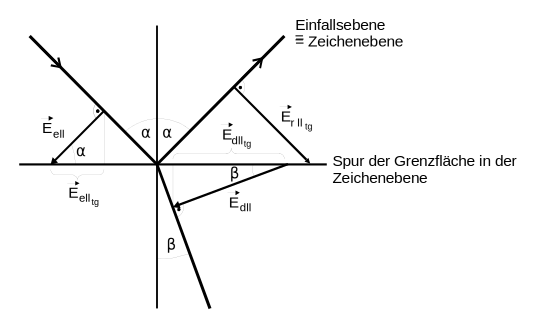
\includegraphics[width=0.8\linewidth]{pictures/grenzfläche3.pdf}
    \caption{Reflexion und Brechung des parallel polarisierten Lichtstrahls. \cite{v407}}
    \label{fig:grenzflaeche3}
\end{figure}

Die Tangentialkomponenten ergeben sich dabei zu
\begin{align*}
    \vec{E}_{\mathrm{e} \| \mathrm{tg}} &= \vec{E}_{\mathrm{e} \|} \cos (\alpha) \, , \\
     \quad \vec{E}_{\mathrm{r} \| \operatorname{tg}} &= -\vec{E}_{\mathrm{r} \|} \cos (\alpha) \quad \text{und} \\ 
     \vec{E}_{\mathrm{d} \| \operatorname{tg}} &= \vec{E}_{\mathrm{d} \|} \cos (\beta) \, .
\end{align*}
Mithilfe der Stetigkeitsbedingung
\begin{equation*}
    \vec{E}_{\mathrm{e} \| \operatorname{tg}}+\vec{E}_{\mathrm{r} \| \mathrm{tg}}=\vec{E}_{\mathrm{d} \| \mathrm{tg}}
\end{equation*}
beziehungsweise
\begin{equation}
    \left(\vec{E}_{\mathrm{e} \|}-\vec{E}_{\mathrm{r} \|}\right) \cos (\alpha)=\vec{E}_{\mathrm{d} \|} \cos (\beta)
\end{equation}
wird \autoref{eq:energiesatz3} zu
\begin{equation} \label{eq:reflektiert}
    \vec{E}_{\mathrm{r} \|} 
    = \vec{E}_{\mathrm{e} \|} \frac{n \cos (\alpha)-\cos (\beta)}{n \cos (\alpha)+\cos (\beta)}
    = \vec{E}_{\mathrm{r} \|}=\vec{E}_{\mathrm{e} \|} \frac{\tan (\alpha-\beta)}{\tan (\alpha+\beta)}
\end{equation}
oder erneut mit dem Snelliuschen Gesetz in \autoref{eq:snellius}
\begin{equation} \label{eq:r_parallel}
    \vec{E}_{\mathrm{r} \|}(\alpha)=\vec{E}_{\mathrm{e} \|} \frac{n^{2} \cos \left(\alpha-\sqrt{n^{2}-\sin ^{2}(\alpha)}\right)}{n^{2} \cos (\alpha)+\sqrt{n^{2}-\sin ^{2}(\alpha)}} \, .
\end{equation}
Hierbei gilt für $\alpha = 0$ und $\alpha = \frac{\pi}{2}$
\begin{align*}
    \vec{E}_{\mathrm{r} \|}(0)=\vec{E}_{\mathrm{e} \|} \frac{n-1}{n+1} 
    \quad \text{und} \quad
    \vec{E}_{\mathrm{r} \|}\left(\frac{\pi}{2}\right)=-\vec{E}_{\mathrm{e} \|} \, .
\end{align*}
Nach \autoref{eq:reflektiert} ergibt sich für
\begin{align*}
    \alpha_{p} + \beta_{p} = \frac{\pi}{2} \vec{E}_{\mathrm{r} \|}\left(\alpha_{p}\right) = 0 \\
    \intertext{und nach dem Snelliuschen Gesetz in \autoref{eq:snellius} folgt demnach}
    n = \tan \left(\alpha_{\text{p}}\right) \, .
\end{align*}
Dabei wird der Winkel $\alpha_\text{p}$ als \textit{Brewsterwinkel} bezeichnet,
der derjenige Winkel ist, ab kein Licht mehr reflektiert wird, sondern vollständig vom Medium absorbiert wird.  